\section*{Third Design}
The third design introduces an effort to decrease the critical path but placing registers after the multipliers. The reset signal is re-introduced in this design iteration in order to eliminate any possiblitiy that this modification to the simulation program may be skewing the output; though it is believed that this is very unlikely.
\subsection*{Pipeling the Critical Path}
The multiplier code has been altered in this design from the simple Verilog library multiplier to include the clocked storage of the output value. The removes the need to create a seperate module for a sixteen bit register. An eight bit register module is still required for the feed back after truncation.  
\\*
`timescale 100ns / 1ns\\*
module mult8(a, b, p, clk, reset);\\*
output signed [15:0] p;\\*
input	clk, reset;\\*
input signed [7:0] a;\\*
input signed [7:0] b;\\*
\\*
reg signed [15:0] p;\\*
wire signed	[15:0] mult_out;\\*
\\*
assign mult_out = a * b;\\*
\\*
always@(posedge clk)\\*
begin\\*
	if(reset == 1'b1) begin\\*
		p <= 16'b0;\\*
	end else begin\\*
		p <= mult_out;\\*
	end\\*
end\\*
\\*
endmodule\\*

\newpage

\subsection*{Third Design Timing Analysis}

% Table generated by Excel2LaTeX from sheet 'Sheet1'
\begin{table}[bh]
\caption{Xilinx Timing Report}
\begin{tabular}{c|c}
\centering
           & Timing in (ns) \\
\hline
     Delay &  17.962   \\

Requrement &      100.000  \\

Data Path Delay &   17.951  \\
\end{tabular}  
\label{tab:timing3}
\end{table}

According to Table \ref{tab:timing3}, the maximum clock frequency for the this design has been calculated to be approximately: 55.7 MHz. This result is troubling as the goal of this iteration is to reduce the critical path delay and effectively increase the operating clock frequency. In fact, this design has increased the delay. After investigating, it seems that the ripple carry adders in use are the critical path as this design does not use a register between the two sixteen bit adders; refer to Figure \ref{subfig:block3-a}. Again, the output waveform is largely ineffective in terms of filtering out high frequencies; refer to Figure \ref{subfig:block3-b} to review the results. 

\begin{figure}[htp]
  \begin{center}
    \subfigure[Functional block diagram]{\label{subfig:block3-a}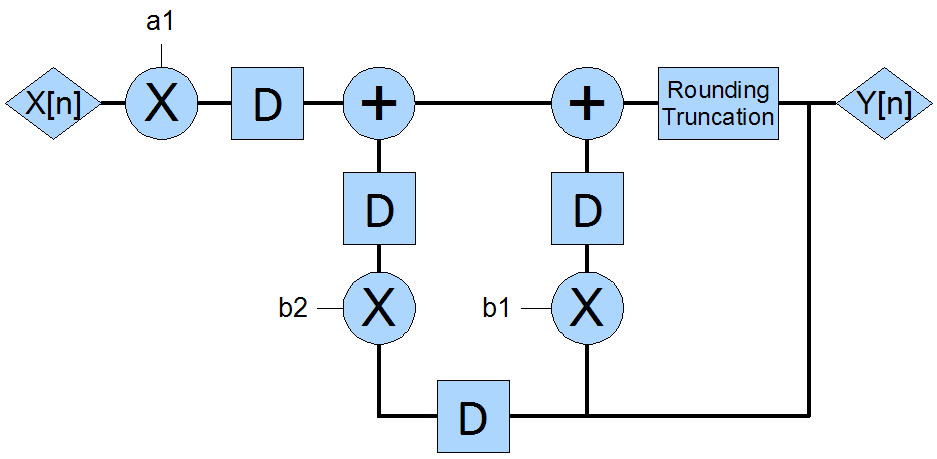
\includegraphics[scale=0.30]{block_three.png}}
    \subfigure[Input/Output comparison]{\label{subfig:output3-b}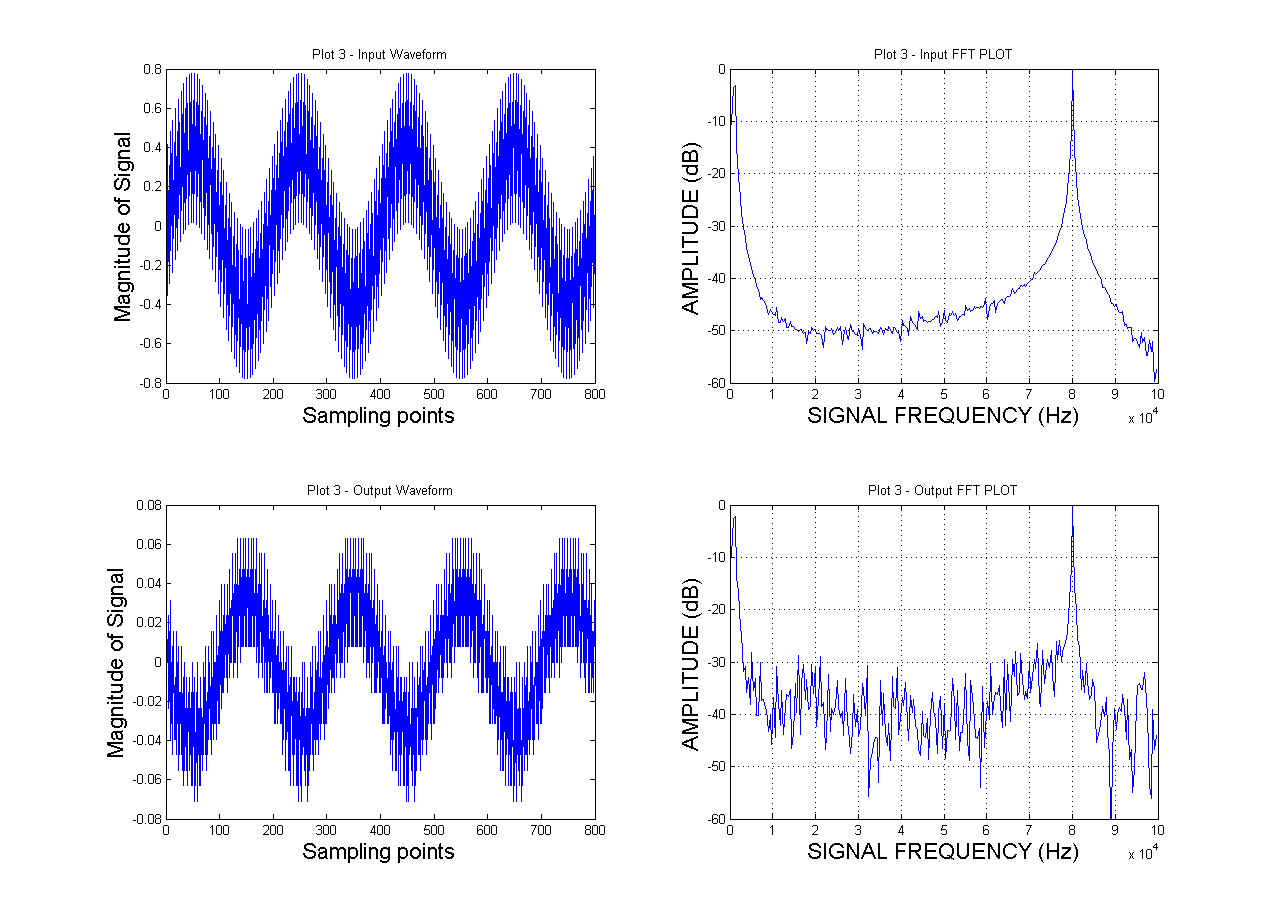
\includegraphics[scale=0.30]{plot3.png}} \\*
  \end{center}
  \caption{Second Design Results}
  \label{fig:design3_results}
\end{figure}